%% Source of figures/empirical-tests.pdf. Compile: pdflatex empirical-tests.tex
%% Generated 2026-10-28 from the SMOTE25 evaluation draft page (76 coded papers, 71 empirical).
%% Numbers are filled from the coded data; regenerate instead of editing them by hand.
\documentclass[border=4pt]{standalone}
\usepackage[scaled]{helvet}\renewcommand{\familydefault}{\sfdefault}
\usepackage{pgfplots}\pgfplotsset{compat=1.18}
\definecolor{sOne}{HTML}{2A78D6}\definecolor{sTwo}{HTML}{EB6834}\definecolor{sThree}{HTML}{1BAF7A}\definecolor{sFour}{HTML}{EDA100}
\definecolor{oZero}{HTML}{A3ABB4}\definecolor{oOne}{HTML}{5598E7}\definecolor{oTwo}{HTML}{1C5CAB}\definecolor{oThree}{HTML}{0D366B}\definecolor{inkTwo}{HTML}{465462}
\begin{document}
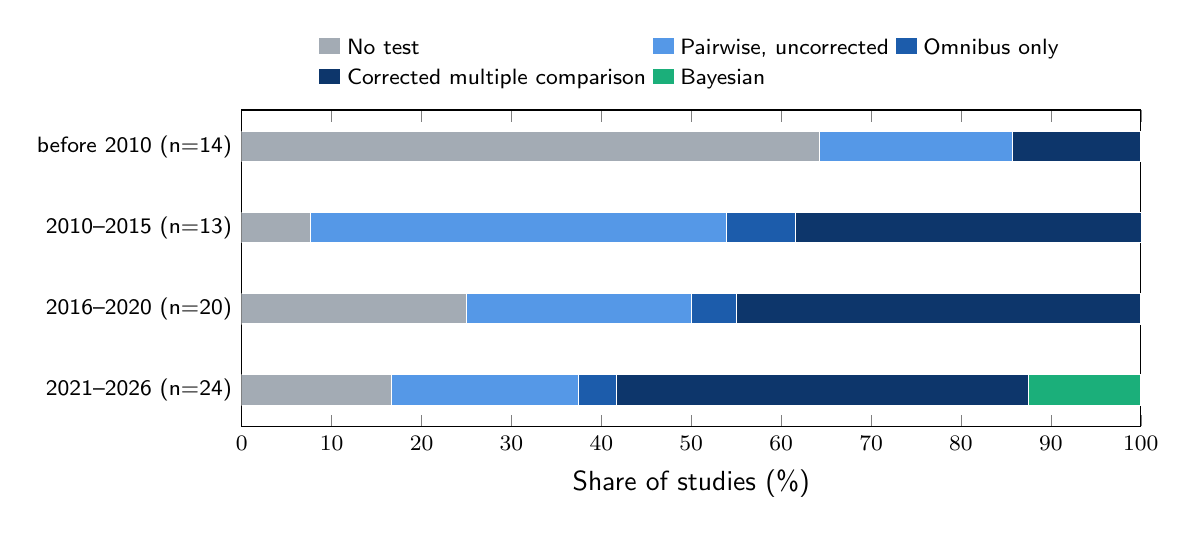
\begin{tikzpicture}
\begin{axis}[xbar stacked,width=13cm,height=5.6cm,bar width=11pt,xmin=0,xmax=100,y dir=reverse,ytick={0,...,3},
  yticklabels={{before 2010 (n=14)},{2010--2015 (n=13)},{2016--2020 (n=20)},{2021--2026 (n=24)}},xlabel={Share of studies (\%)},enlarge y limits=0.15,
  tick label style={font=\footnotesize},legend cell align=left,legend style={font=\footnotesize,at={(0.5,1.03)},anchor=south,legend columns=3,draw=none}]
\addplot[fill=oZero,draw=white] coordinates {(64.3,0) (7.7,1) (25.0,2) (16.7,3)};
\addplot[fill=oOne,draw=white] coordinates {(21.4,0) (46.2,1) (25.0,2) (20.8,3)};
\addplot[fill=oTwo,draw=white] coordinates {(0.0,0) (7.7,1) (5.0,2) (4.2,3)};
\addplot[fill=oThree,draw=white] coordinates {(14.3,0) (38.5,1) (45.0,2) (45.8,3)};
\addplot[fill=sThree,draw=white] coordinates {(0.0,0) (0.0,1) (0.0,2) (12.5,3)};
\legend{{No test},{Pairwise, uncorrected},{Omnibus only},{Corrected multiple comparison},{Bayesian}}
\end{axis}
\end{tikzpicture}
\end{document}
